\section{The reference profile: requirements and solvable models}
\label{sec:rosen-reference-packet}
\label{sec:radial-models}

Part~\ref{part:reference} constructs one radial profile $w_*$ at which
the linearized equation has a single flat infinitesimal bending and a
controlled inverse. This section states precisely what is needed
(Proposition~\ref{prop:rad-fixed-theorem}), explains the layout of the
construction and its vocabulary, and introduces the two explicitly
solvable models from which $w_*$ is assembled.

\subsection{Angular modes and the design problem}

Functions in our symmetry class have the Fourier expansion
\[
 u(r,\theta)=u_0(r)+\sum_{\substack{j\ge2\\ j\ \mathrm{even}}}
 u_j(r)\,e_j(\theta),
 \qquad e_j(\theta)=\sqrt2\cos(j\theta),
\]
and on the $j$th mode the operator \eqref{eq:intro-linearization} acts
as the ordinary differential operator
\begin{equation}\label{eq:rad-eq-modal-operator}
 L_ju=(wu')'-j^2\,\frac{w'}r\,u,
 \qquad\text{that is,}\qquad
 \mathscr L_w(u\,e_j)=(L_ju)\,e_j .
\end{equation}
When the dependence on the profile matters we write $L_{j,w}$. We want
a profile for which
\begin{itemize}
\item at $j=2$ there is exactly one solution of $L_2\phi=0$, up to
 multiples, which is flat at both endpoints. This is the seed of the
 nonradial height. The frequency two is the lowest one compatible with
 the half-turn symmetry required in
 Theorem~\ref{thm:geometric-closure};
\item at every even $j\ge4$ there is no such solution, and $L_j$ has a
 controlled inverse. The nonlinear equation creates all higher even
 frequencies, so all of them must be invertible on the same profile.
\end{itemize}

Two freedoms are available, and separating them is the organizing idea
of the construction. The \emph{shape} of a piece of the profile
determines the homogeneous solutions on that piece, hence its spectrum
and its travel angles. Multiplying a piece by a positive constant, its
\emph{height}, changes none of these, but it changes the scale of the
flux $wu'$ by which solutions on neighbouring pieces are compared. We
use the first freedom to make each piece explicitly solvable, and the
second to prevent resonances when the pieces are joined.

\subsection{What the reference profile must provide}
\label{sec:radial-what}

We state the result of Part~\ref{part:reference} before starting the
construction. It involves three scales attached to the $n$th piece of
the profile near an endpoint.

\begin{definition}[The endpoint scales]\label{def:radial-weights}
The pieces of the profile approaching either endpoint are called
\emph{cells} and are indexed by integers $n\ge N$. We set
\begin{equation}\label{eq:rad-eq-endpoint-weights}
 A_n\asymp e^{-n^2},\qquad
 S_n=\tfrac23\,n^3,\quad H_n=e^{-S_n},\qquad
 q_n=n^{5/2}\log(e+n),\quad \mathcal E_n=e^{q_n}.
\end{equation}
\begin{itemize}
\item $A_n$ is the \emph{length scale}: cell $n$ has radial length
 comparable to $A_n$.
\item $H_n$ is the \emph{decay scale}: the distinguished solution of
 $L_j u=0$ at the endpoint decays like $H_n$ across the cells.
\item $\mathcal E_n$ is the \emph{coefficient allowance}: reciprocals
 and derivatives of the coefficients on cell $n$ are bounded by powers
 of $\mathcal E_n$.
\end{itemize}
A bound of the form $C\mathcal E_n^{C}$ is called a \emph{coefficient
power}; a \emph{coefficient estimate of order $s$} on cell $n$ is a
bound by $C_s\mathcal E_n^{C_s}$. On the finitely many pieces in the
middle of the annulus the same words refer to fixed positive
constants. For the purpose of estimates a cell includes fixed portions
of its neighbours; such an enlargement changes the index by a bounded
amount, which is immaterial.
\end{definition}

The three scales are ordered: for all fixed $a,b,\varepsilon>0$,
\begin{equation}\label{eq:rad-scale-separation}
 \mathcal E_n^{a}\,e^{bn^2}\le C_{a,b,\varepsilon}\,e^{\varepsilon S_n},
 \qquad\text{because}\qquad n^2=o(q_n),\quad q_n=o(S_n).
\end{equation}
So lengths are much larger than coefficient allowances, which are much
larger than the decay scale. Section~\ref{sec:radial-tails} derives all
three scales from the construction; they are not hypotheses about an
unknown profile.

\paragraph{Weighted norms.}
Choose a smooth partition of unity $\vartheta_m$ on $(r_-,r_+)$ with
bounded overlap, subordinate to the cells of both tails and to the
finite middle part; the index $m$ records both the endpoint and the
cell. Fix a smooth function $\chi_L$ of $r$ equal to one near the left
endpoint and to zero near the right one. For exponents $0<\gamma<1$
and $\ea\ge0$, the \emph{source norm} of a pair $(f,c)$, consisting of
a function $f$ and a scalar $c$, is
\begin{equation}\label{eq:rad-eq-source-norm}
 \|(f,c)\|_{Y_{\gamma,s}}^2
 =|c|^2+\sum_m\mathcal E_m^{2\ea}H_m^{-2\gamma}
       \|\vartheta_m f\|_{L^2(dr)H^s(\T)}^2 .
\end{equation}
The \emph{output norm} is defined for pairs $(u,\nu)$ of a function
and a scalar. Write $u=a_L\chi_L+v$ with a constant $a_L$; then the
squared output norm is
\[
 |a_L|^2+|\nu|^2+\sum_m\mathcal E_m^{-2\eb}H_m^{-2\gamma}
       \|\vartheta_m v\|_{L^2(dr\,d\theta)}^2 .
\]
A finite source norm means decay like $H_m^{\gamma}$ towards the
endpoints, with $\ea$ powers of the coefficient allowance to spare. A
finite output norm means the same decay for $v$, after the loss of
$\ea+\eb$ such powers, while $u$ itself tends to $a_L$ at the left
endpoint and to $0$ at the right one.

\begin{proposition}[The reference profile]\label{prop:rad-fixed-theorem}
There are radii $0<r_-<r_+$ and a smooth function $w_*>0$ on
$(r_-,r_+)$, flat at both endpoints, such that all zeros of $w_*'$ in
$(r_-,r_+)$ are simple, with the following properties.
\begin{enumerate}
\item \textup{(Kernel.)} There is a nonzero function $\phi_*$, flat at
 both endpoints, with $L_{2,w_*}\phi_*=0$. It spans the endpoint-flat
 kernel of $L_{2,w_*}$, and the endpoint-flat kernel of $L_{j,w_*}$ is
 zero for every even $j\ge4$.
\item \textup{(Travel angles.)} For every component $m$ of
 $\{w_*'<0\}$ the travel angle
 $T_m=\int\sqrt{-w_*'/(rw_*)}\,dr$ over that component satisfies
 \begin{equation}\label{eq:rad-eq-optical-margin}
  |\sin(kT_m)|\ge\frac{\gamma_m}{k}\quad(k\ge1),
  \qquad \gamma_m^{-1}\le\mathcal E_m^{C},
  \qquad T_m/\pi\ \text{is a quadratic irrational}.
 \end{equation}
\item \textup{(Border.)} There is a smooth function $\chi_*$,
 compactly supported in a component of $\{w_*'>0\}$, such that
 \begin{equation}\label{eq:rad-eq-target-border}
  g_*=L'_{2,w_*}[w_*\chi_*]\,\phi_*,\qquad
  \int g_*\phi_*\,dr=1,\qquad
  \ell_*u=\int g_*u_2\,dr .
 \end{equation}
 Here $L'_{2,w}[\omega]\phi=(\omega\phi')'-4\omega'\phi/r$ is the
 derivative of $L_{2,w}\phi$ with respect to the profile $w$ in the
 direction $\omega$.
\item \textup{(Inverse.)} The bordered operator
 \begin{equation}\label{eq:rad-eq-bordered-reference}
  \mathbb L_{w_*}(u,\nu)
    =\bigl(\mathscr L_{w_*}u+\nu\,g_*e_2,\ \ell_*u\bigr)
 \end{equation}
 has a two-sided inverse on the sources $(f,c)$ satisfying the
 compatibility condition $\int\av f\,dr=0$, where $u$ is required to
 tend to zero at the right endpoint and to an arbitrary constant at
 the left one. For every compact interval
 $[\gamma_-,\gamma_+]\subset(0,1)$ there are exponents $\ea,\eb$ such
 that this inverse is bounded from $Y_{\gamma,0}$ to the output norm,
 uniformly for $\gamma\in[\gamma_-,\gamma_+]$. One radial derivative
 of the output costs at most one additional angular derivative of the
 source.
\item \textup{(Independence of the exponent.)} The profile, the
 function $\phi_*$ and the border are the same for all exponents
 $\gamma$.
\end{enumerate}
\end{proposition}

Some comments on the statement.

\emph{The border.} Since $L_2$ has a one-dimensional kernel, and is
formally symmetric, it has a one-dimensional cokernel as well. The
standard remedy is to \emph{border} the operator: one adds a scalar
unknown $\nu$ multiplying a fixed function $g_*$ (the \emph{column})
and a scalar equation $\ell_*u=c$ (the \emph{row}). The column removes
the cokernel and the row removes the kernel. Our column has a
meaning: if the profile is deformed to $w_*e^{\nu\chi_*}$, then
$g_*e_2$ is the derivative of
$\mathscr L_w(\phi_*e_2)$ with respect to $\nu$. So $\nu$ will be an
actual parameter of the metric in the nonlinear problem.

\emph{The compatibility condition and the free constant.} These
concern the mode $j=0$, where $L_0u=(wu')'$. By
Lemma~\ref{lem:scalar-integral} the sources of interest have
$\int\av f\,dr=0$; and the difference of the two endpoint values of
the height is not prescribed.

\emph{Endpoint-flat kernel.} The precise meaning of this term, and of
the two-sided inverse, is given by the weighted graph domain of
Definition~\ref{def:radial-graph-domain}.

\emph{What is proved here, and what later.}
Proposition~\ref{prop:rad-fixed-theorem} is an estimate at angular
order zero, together with its first radial derivative. Estimates of
all orders are recovered from the differential equation in
Section~\ref{sec:stable-inverse}, after the weighted spaces of the
nonlinear problem have been introduced. Keeping the two tasks apart
means that the geometry of the profile does not depend on the order
of regularity.

The proof of Proposition~\ref{prop:rad-fixed-theorem} occupies the
rest of this section and the next two; it is completed in
Section~\ref{subsec:final-border}.

\subsection{Layout of the construction and vocabulary}
\label{subsec:layout}

Figure~\ref{fig:layout} shows how $w_*$ is assembled. The following
terms are used throughout Parts~\ref{part:reference}
and~\ref{part:nonlinear}.

\begin{figure}[htbp]
\centering
\begin{tikzpicture}[x=1cm,y=1cm,>=Stealth,font=\small]
\draw[->] (-.3,0)--(13.3,0) node[right] {$r$};
\draw[fill=blue!13] (0,.3) rectangle (3.4,.95);
\draw[fill=gray!15] (3.4,.3) rectangle (5.3,.95);
\draw[fill=orange!22] (5.3,.3) rectangle (7.7,.95);
\draw[fill=gray!15] (7.7,.3) rectangle (9.6,.95);
\draw[fill=blue!13] (9.6,.3) rectangle (13,.95);
\node at (2.3,.62) {left tail};
\node at (4.35,.62) {cones};
\node at (6.5,.62) {central model};
\node at (8.65,.62) {cones};
\node at (10.7,.62) {right tail};
\foreach \x in {.12,.27,.47,.75,1.15}{\draw (\x,.3)--(\x,.95);}
\foreach \x in {12.88,12.73,12.53,12.25,11.85}{\draw (\x,.3)--(\x,.95);}
\node[below] at (0,-.05) {$r_-$};
\node[below] at (13,-.05) {$r_+$};
\node[align=center] at (1.7,1.55) {cells $\ldots,N+1,N$\\(Morse models)};
\node[align=center] at (11.3,1.55) {cells $N,N+1,\ldots$\\(Morse models)};
\node[align=center] at (6.5,1.55) {harmonic oscillator:\\carries the seed $\phi_*$};
\node[align=center] at (4.35,-.75) {$w=cr$ and\\connectors};
\node[align=center] at (8.65,-.75) {$w=cr$ and\\connectors};
\draw[->] (4.35,-.35)--(4.35,.25);
\draw[->] (8.65,-.35)--(8.65,.25);
\end{tikzpicture}
\caption{The layout of the reference profile $w_*$ (schematic). The
cells shrink and accumulate at both endpoints. Consecutive pieces are
separated by intervals on which $w_*'>0$.}
\label{fig:layout}
\end{figure}

\begin{description}[leftmargin=1.5em,style=sameline,font=\normalfont\itshape]
\item[Positive and negative components.] A \emph{positive component}
 is a component of $\{w'>0\}$; the equation is elliptic there. A
 \emph{negative component} is a component of $\{w'<0\}$; the equation
 is hyperbolic there. They are separated by the turning circles, also
 called \emph{roots}.
\item[Travel angle.] The travel angle of a negative component is
 $T=\int\sqrt{-w'/(rw)}\,dr$ over that component: the angle by which a
 characteristic of $\mathscr L_w$ turns while crossing it.
\item[Model.] A piece of the profile on which, in a suitable
 \emph{model coordinate} $X$, every $L_j$ is conjugate to an
 explicitly solvable Schr\"odinger operator
 (Section~\ref{subsec:liouville}). There are two kinds: the
 \emph{central model} and the Morse \emph{cells}.
\item[Cell.] The $n$th cell consists, in the direction of increasing
 $r$, of a \emph{short positive cap}, one negative component, and a
 \emph{long positive cap} (Figure~\ref{fig:cell}).
\item[Join.] A very short positive interval between two consecutive
 cells, on which $w$ rises steeply from the height of one cell to that
 of the next.
\item[Cone.] An interval on which $w=cr$. There
 $L_ju=c\,[(ru')'-j^2u/r]$ has the solutions $r^{\pm j}$.
\item[Connector.] A positive interval joining the central model or a
 tail to a cone, built so that the seed solution is preserved exactly
 (Section~\ref{subsec:rad-cone-bump-target-match}).
\item[Tail.] The union of the cells and joins near one endpoint.
\item[Buffer.] A positive interval, viewed as a region across which
 the solutions of $L_ju=0$ grow or decay exponentially; it decouples
 the pieces on its two sides.
\item[Natural line, incoming line.] At a point of a tail, and for a
 fixed frequency $j$, the \emph{natural line} is the one-dimensional
 space of solutions of $L_ju=0$ that decay towards the endpoint
 (Lemma~\ref{lem:radial-deep-inverse}). The \emph{incoming line} is
 the one-dimensional space of solutions satisfying the condition
 imposed on the interior side. A homogeneous solution of the whole
 problem exists exactly when the two lines coincide.
\item[Outward.] Towards the nearer endpoint.
\end{description}

The plan of Part~\ref{part:reference} is as follows.
\begin{itemize}
\item Section~\ref{subsec:liouville} explains how a Schr\"odinger
 potential determines a radial profile.
 Sections~\ref{subsec:rad-central-singlepoint}
 and~\ref{subsec:morse} treat the central model and the Morse model on
 the whole line: spectrum, spectral gap at energy zero, travel angle.
\item Section~\ref{sec:radial-tails} builds the tails. It proves that
 at every frequency the natural line exists, is unique, and consists
 of flat functions, and it chooses the heights of the cells so that
 natural and incoming lines stay apart.
\item Section~\ref{sec:radial-reference-inverse} joins all pieces and
 proves that the local information combines to an inverse on the whole
 annulus.
\end{itemize}

\subsection{From a Schr\"odinger potential to a radial profile}
\label{subsec:liouville}

It is easier to design the spectrum first and the radius afterwards.

\begin{lemma}[Liouville transformation]\label{lem:liouville}
Let $X$ range over an interval, let $r(X)$ be a smooth function with
$r>0$ and $r_X>0$, let $\mathcal P(X)>0$ be smooth, and let
$\lambda>0$. Define a profile $w$ and two functions $\rho,V_0$ of $X$
by
\begin{equation}\label{eq:rad-eq-sc0}
 w(r(X))=\lambda\,\mathcal P(X)\,r_X(X),\qquad
 \rho=-\frac{r_{XX}+(\mathcal P_X/\mathcal P)\,r_X}{r},\qquad
 V_0=\frac{(\sqrt{\mathcal P})_{XX}}{\sqrt{\mathcal P}} .
\end{equation}
Then $w'=-\lambda\mathcal P\rho\,r/r_X$, and for every $j$ and every
function $\psi(X)$,
\begin{equation}\label{eq:liouville-identity}
 L_j\bigl(\mathcal P^{-1/2}\psi\bigr)
   =-\frac{\lambda\sqrt{\mathcal P}}{r_X}\,
      \bigl(-\psi_{XX}+(V_0-j^2\rho)\,\psi\bigr).
\end{equation}
\end{lemma}

\begin{proof}
For a function $u$ of $r$ we have $wu_r=\lambda\mathcal Pu_X$, hence
$(wu_r)_r=\lambda(\mathcal Pu_X)_X/r_X$. Differentiating
$w=\lambda\mathcal Pr_X$ and using the definition of $\rho$ gives the
formula for $w'$. Therefore
$L_ju=(\lambda/r_X)\,[(\mathcal Pu_X)_X+j^2\mathcal P\rho\,u]$, and
with $u=\mathcal P^{-1/2}\psi$ one has
$(\mathcal Pu_X)_X=\sqrt{\mathcal P}\,(\psi_{XX}-V_0\psi)$.
\end{proof}

We use the lemma in the opposite direction. Given a density
$\mathcal P$ and a function $\rho$, the homogeneous equation
$L_ju=0$ is equivalent to the Schr\"odinger equation
\[
 H_j\psi:=-\psi_{XX}+(V_0-j^2\rho)\,\psi=0 ,
\]
\emph{provided} the linear equation
$r_{XX}+(\mathcal P_X/\mathcal P)\,r_X+\rho\,r=0$ for the radius has a
solution which is positive and increasing. Three features of the
dictionary are used constantly.
\begin{itemize}
\item The height $\lambda$ does not enter the homogeneous equation.
\item The profile is falling where $\rho>0$ and rising where $\rho<0$.
 The negative components are the components of $\{\rho>0\}$, the
 turning circles are the zeros of $\rho$, and the travel angle of a
 negative component is
 \begin{equation}\label{eq:travel-angle-model}
  T=\int\sqrt{-w'/(rw)}\,dr=\int_{\{\rho>0\}}\sqrt\rho\,dX .
 \end{equation}
\item Frequency enters only through the coupling constant $j^2$ in
 front of $\rho$.
\end{itemize}

We use two potentials with complementary roles
(Figure~\ref{fig:two-spectral-models}). The harmonic oscillator, in
the middle, has a zero mode at $j=2$ and is used to create the seed.
The Morse potential, near the ends, has a spectral gap at energy zero
for all $j$, and its cells are short enough in radius to accumulate at
a finite point. It is the explicit spectra of the two models, not
merely the shapes of their potentials, that make them useful.

\begin{figure}[htbp]
\centering
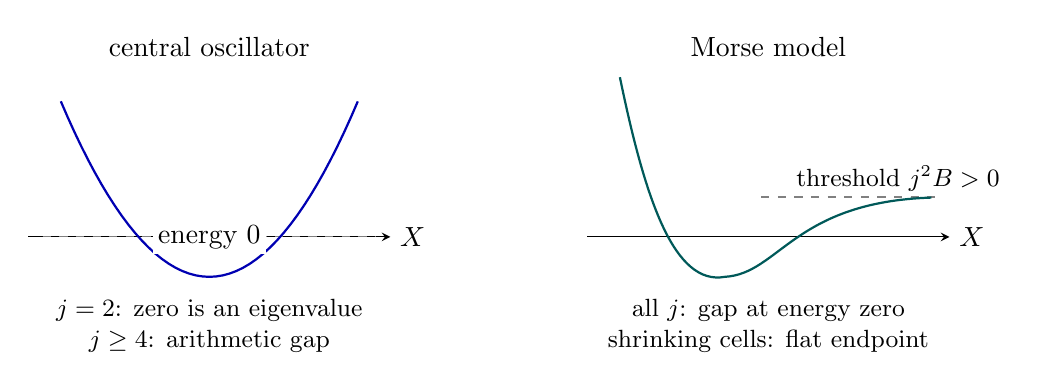
\begin{tikzpicture}[x=.92cm,y=.78cm,>=stealth]
\begin{scope}
\draw[->] (-2.5,0)--(2.5,0) node[right] {$X$};
\draw[dashed,gray] (-2.3,0)--(2.3,0);
\draw[thick,blue!70!black,domain=-2.05:2.05,samples=45]
 plot (\x,{.68*\x*\x-.65});
\node[align=center] at (0,3.1) {central oscillator};
\node[fill=white,inner sep=2pt] at (0,0) {energy $0$};
\node[align=center,font=\small] at (0,-1.45)
 {$j=2$: zero is an eigenvalue\\$j\ge4$: arithmetic gap};
\end{scope}
\begin{scope}[xshift=7.1cm]
\draw[->] (-2.5,0)--(2.5,0) node[right] {$X$};
\draw[dashed,gray] (-.1,.65)--(2.3,.65);
\draw[thick,teal!70!black]
 (-2.05,2.6) .. controls (-1.7,.6) and (-1.3,-.8) .. (-.6,-.65)
 .. controls (.15,-.6) and (.35,.57) .. (2.25,.64);
\node[align=center] at (0,3.1) {Morse model};
\node[anchor=west,font=\small] at (.25,.95) {threshold $j^2B>0$};
\node[align=center,font=\small] at (0,-1.45)
 {all $j$: gap at energy zero\\shrinking cells: flat endpoint};
\end{scope}
\end{tikzpicture}
\caption{The potentials $V_0-j^2\rho$ of the two models on the whole
line, drawn schematically with an arbitrary vertical scale. Only
finite pieces of them are used in the profile, and the pieces are
separated by regions where the potential is positive.}
\label{fig:two-spectral-models}
\end{figure}

\subsection{The central oscillator}
\label{subsec:rad-central-singlepoint}

\paragraph{Definition and spectrum.}
Fix the constants
\begin{equation}\label{eq:rad-eq-sc1}
 A_c=\frac1{\sqrt2},\qquad a_c=\sqrt{4A_c-2},\qquad
 c_c=3A_c-2>0,\qquad \alpha_c=\frac{c_c+1}2,
\end{equation}
and take
\[
 \mathcal P=e^{-2a_cX},\qquad \rho=A_c-X^2 .
\]
Then $V_0=a_c^2$, and the Schr\"odinger operator of
Lemma~\ref{lem:liouville} is a shifted harmonic oscillator,
\[
 H_{j,c}=-\partial_X^2+j^2X^2+a_c^2-j^2A_c ,
\]
with eigenvalues \cite[\S8.3, equations (8.33)--(8.42)]{Teschl2009}
\begin{equation}\label{eq:central-spectrum-new}
 E_{m,j}=j(2m+1)+a_c^2-j^2A_c,\qquad m=0,1,2,\ldots
\end{equation}
The value of $a_c$ is chosen so that $E_{0,2}=0$: at $j=2$ the
eigenvalues are $E_{m,2}=4m$, and the kernel is spanned by the ground
state $e^{-X^2}$. The irrationality of $A_c$ keeps all other even
frequencies away from zero:

\begin{lemma}[Spectral gap of the central model]\label{lem:central-gap}
Let $\delta_c=\tfrac34(3-2\sqrt2)>0$. Then
\begin{equation}\label{eq:rad-eq-sc3}
 \|H_{j,c}^{-1}\|\le\frac2{\delta_c}\quad(j\ge4\ \text{even}),
 \qquad \ker H_{2,c}=\operatorname{span}\{e^{-X^2}\},
\end{equation}
and the inverse of $H_{2,c}$ on the orthogonal complement of its
kernel has norm $1/4$. Here $H_{j,c}$ is the self-adjoint operator on
$L^2(\R)$ defined by its closed quadratic form.
\end{lemma}

\begin{proof}
Only the first bound needs proof; it says $|E_{m,j}|\ge\delta_c/2$ for
even $j\ge4$. Put $\Phi_j=jA_c-a_c^2/j$, so that
$E_{m,j}=j\,(2m+1-\Phi_j)$. Since $A_c^2=\tfrac12$,
\[
 N_j:=\frac{j^2}2-\Phi_j^2=2A_ca_c^2-\frac{a_c^4}{j^2}
 \in\Bigl[\tfrac{13}4-\tfrac{3\sqrt2}2,\ 4-2\sqrt2\Bigr)
 \qquad(j\ge4),
\]
and this interval lies in $(1,2)$ at distance $\delta_c$ from the
integers. Suppose $|E_{m,j}|<1$. Then $2m+1+\Phi_j<2j$, and because
$j^2/2-(2m+1)^2$ is an integer,
\[
 \delta_c\le\bigl|(2m+1)^2-\Phi_j^2\bigr|
 =\frac{|E_{m,j}|}{j}\,(2m+1+\Phi_j)<2\,|E_{m,j}| .
\]
If $|E_{m,j}|\ge1$ there is nothing to prove.
\end{proof}

\paragraph{The model is a radial profile.}
We need a positive increasing solution of the radius equation, which
for the present $\mathcal P$ and $\rho$ reads
$r_{XX}-2a_cr_X+(A_c-X^2)\,r=0$. An arbitrary solution would not do;
here is an explicit one.

\begin{lemma}[The central radius]\label{lem:central-radius}
Let
\begin{equation}\label{eq:rad-eq-sc6}
 \psi_1(X)=e^{-X^2/2}\int_0^\infty
 t^{\alpha_c-1}e^{-t^2/2+\sqrt2\,Xt}\,dt,
 \qquad r=e^{a_cX}\psi_1,\qquad \upsilon=\frac{r_X}r .
\end{equation}
Then $r$ is a positive solution of the radius equation, increasing
from $0$ to $\infty$, with $\upsilon>a_c$. Moreover
\begin{equation}\label{eq:rad-eq-sc6a}
 \upsilon=
 \begin{cases}
 -X+a_c-\alpha_c/X+O(X^{-3}),&X\to-\infty,\\[2pt]
 \phantom{-}X+a_c+(\alpha_c-1)/X+O(X^{-3}),&X\to+\infty,
 \end{cases}
\end{equation}
and these expansions may be differentiated any fixed number of times.
In particular $\upsilon\asymp1+|X|$.
\end{lemma}

\begin{proof}
An integration by parts in $t$ shows $\psi_1''=(X^2+c_c)\,\psi_1$.
Since $c_c-a_c^2+A_c=0$, the function $r=e^{a_cX}\psi_1$ solves the
radius equation. Clearly $\psi_1>0$, and $\psi_1,\psi_1'\to0$ as
$X\to-\infty$; then $\psi_1''>0$ implies $\psi_1'>0$, so
$\upsilon=a_c+\psi_1'/\psi_1>a_c$.

The leading terms of \eqref{eq:rad-eq-sc6a} can be read off from the
equation: as $|X|\to\infty$ the solutions of
$\psi''=(X^2+c_c)\psi$ behave like $|X|^{\alpha_c-1}e^{X^2/2}$ or like
$|X|^{-\alpha_c}e^{-X^2/2}$, and $\psi_1$ is of the second kind at
$-\infty$ and of the first kind at $+\infty$. To prove the expansions
with their remainders, use the integral.
For the expansion at $X=-L$, substitute $t=z/(\sqrt2L)$: the remaining
integral is $\Gamma(\alpha_c)(1+O(L^{-2}))$ and may be differentiated
under an exponentially integrable majorant. For $X>0$, complete the
square and expand $t^{\alpha_c-1}$ about $t=\sqrt2X$ against the
Gaussian; the region $|t-\sqrt2X|>X/2$ contributes an exponentially
small amount. Logarithmic differentiation gives
\eqref{eq:rad-eq-sc6a}, and with it the range of $r$.
\end{proof}

\paragraph{The seed and the two ends.}
By Lemma~\ref{lem:liouville} the kernel of $H_{2,c}$ corresponds to
the solution
\begin{equation}\label{eq:rad-eq-sc2}
 \phi_0=\mathcal P^{-1/2}e^{-X^2}=e^{a_cX-X^2},\qquad
 \frac{\partial_y\phi_0}{\phi_0}=\frac{a_c-2X}{\upsilon}
 \longrightarrow
 \begin{cases}\phantom{-}2&\text{as }X\to-\infty,\\
              -2&\text{as }X\to+\infty,\end{cases}
\end{equation}
of $L_2\phi_0=0$, where $y=\log r$. So at its two ends $\phi_0$
behaves like the solutions $r^{2}$ and $r^{-2}$ on a cone. The profile
itself also becomes conical: writing $w=re^f$,
\begin{equation}\label{eq:rad-eq-sc6b}
 1+f_y=\frac{rw'}{w}=\frac{X^2-A_c}{\upsilon^2}\longrightarrow1
 \qquad(X\to\pm\infty).
\end{equation}
Both limits hold with any fixed number of $y$-derivatives, by
\eqref{eq:rad-eq-sc6a}. We may therefore cut the model so far out on
both sides that the two end regions are positive, with uniformly
bounded jets in the logarithmic coordinate $y$. The retained piece
contains exactly two turning circles, at $X=\pm\sqrt{A_c}$. By
\eqref{eq:travel-angle-model} its travel angle is
\[
 T=\int_{-\sqrt{A_c}}^{\sqrt{A_c}}\sqrt{A_c-X^2}\,dX
  =\frac{\pi A_c}2=\frac{\pi}{2\sqrt2},
\]
and $|\sin(kT)|\ge c/k$ for all $k\ge1$, because $k^2-8m^2$ is a
nonzero integer for all integers $k\ge1$ and $m$.

\paragraph{The inverse in radial units.}
Estimates in the radial variable are made in a weighted $L^2$ space.
Define
\begin{equation}\label{eq:rad-eq-ha2}
 \varpi=\frac{12\,w}{r^2},\qquad B_j=-\varpi^{-1}L_j,
 \qquad
 \|u\|_{L^2(\varpi\,dr)}^2=12\lambda\,\|\upsilon\psi\|_{L^2(dX)}^2
 \quad\text{for }u=\mathcal P^{-1/2}\psi .
\end{equation}
The operator $B_j$ is symmetric in $L^2(\varpi\,dr)$, and on a cone it
is $\tfrac1{12}(-\partial_y^2+j^2)$. By \eqref{eq:liouville-identity},
$B_j$ corresponds to $\tfrac1{12}\upsilon^{-2}H_{j,c}$, so in the
variable $\upsilon\psi$ its inverse is
$12\,\upsilon H_{j,c}^{-1}\upsilon$, not merely $H_{j,c}^{-1}$.

\begin{lemma}\label{lem:central-weighted}
The operators $\upsilon H_{j,c}^{-1}\upsilon$, $j\ge4$ even, are
bounded on $L^2(dX)$ uniformly in $j$. The same holds at $j=2$ for the
inverse on the complement of the kernel.
\end{lemma}

\begin{proof}
The potential $V_j=j^2X^2+a_c^2-j^2A_c$ satisfies
$V_j\ge cj^2\upsilon^2-Cj^2$. For $\psi=H_{j,c}^{-1}G$ this and
Lemma~\ref{lem:central-gap} give
$cj^2\|\upsilon\psi\|^2\le\langle G,\psi\rangle+Cj^2\|\psi\|^2
 \le Cj^2\|G\|^2$,
so $\|\upsilon H_{j,c}^{-1}\|\le C$, and by taking adjoints
$\|H_{j,c}^{-1}\upsilon\|\le C$. Now let
$\psi=H_{j,c}^{-1}(\upsilon F)$. In the same way
\[
 cj^2\|\upsilon\psi\|_2^2
 \le\|\upsilon\psi\|_2\|F\|_2+Cj^2\|F\|_2^2 ,
\]
and absorbing the first term on the right proves the claim. At $j=2$,
add to $H_{2,c}$ the orthogonal projection onto $e^{-X^2}$, apply the
same argument, and subtract the projection, whose weighted norm is
finite.
\end{proof}

\paragraph{A temporary border.}
During the construction, mode two of the central model is bordered by
a compactly supported function $g_0$ with $\int g_0\phi_0\,dr=1$ and
by the row $\ell_0u=\int g_0u\,dr$. A source is made orthogonal to
$\phi_0$ by subtracting a multiple of $g_0$, and the row is fulfilled
by adding a multiple of $\phi_0$; so the bordered inverse obeys the
bounds of Lemma~\ref{lem:central-weighted}. The scalar is normalized
so that under a rescaling $w\mapsto\lambda w$ of the height one has
$g_0\mapsto\sqrt\lambda\,g_0$ and $\phi_0\mapsto\phi_0/\sqrt\lambda$;
then row and column have bounded norms in the Hilbert space
$L^2(\varpi\,dr)$. This auxiliary border is replaced by the final one
\eqref{eq:rad-eq-target-border} in
Section~\ref{subsec:final-border}, after all geometric choices have
been made.

\subsection{The Morse model}
\label{subsec:morse}

\paragraph{Definition and spectrum.}
For the tails take $\mathcal P=1$, so $V_0=0$, and for parameters
$A>4B>0$
\[
 \rho(X)=A\,(e^{-X}-e^{-2X})-B,
 \qquad H_{j,M}=-\partial_X^2-j^2\rho .
\]
The potential $-j^2\rho$ is confining as $X\to-\infty$ and tends to
$j^2B$ exponentially as $X\to+\infty$. Hence the essential spectrum of
$H_{j,M}$ is $[j^2B,\infty)$ \cite[Theorem~6.19]{Teschl2009}. Below it
there are finitely many simple eigenvalues, given by Morse's formula
\cite{Morse1929}
\begin{equation}\label{eq:rad-eq-fs1}
 E_{m,j}=j^2B-(\alpha_j-m)^2,
 \qquad \alpha_j=\frac{j\sqrt A-1}2,\qquad 0\le m<\alpha_j .
\end{equation}
For completeness we recall the factorization which proves
\eqref{eq:rad-eq-fs1} and fixes its normalization. Let
$\omega=j\sqrt A$, and for real $\alpha$ put
\[
 D_\alpha=\partial_X+\alpha-\omega e^{-X},\qquad
 H_\alpha=-\partial_X^2+\omega^2e^{-2X}-(2\alpha+1)\,\omega e^{-X}+j^2B,
\]
so that $H_{j,M}=H_{\alpha_j}$. A direct computation gives
\[
 H_\alpha=D_\alpha^*D_\alpha+j^2B-\alpha^2,
 \qquad
 H_{\alpha-1}=D_\alpha D_\alpha^*+j^2B-\alpha^2 .
\]
The null function of $D_\alpha$ is $e^{-\alpha X-\omega e^{-X}}$,
which is square integrable exactly when $\alpha>0$. Passing from
$H_\alpha$ to $H_{\alpha-1}$ thus removes the ground state
$j^2B-\alpha^2$ and keeps the rest of the spectrum. For
$-1<\alpha\le0$ one has
$H_\alpha-j^2B=D_0^*D_0-2\omega\alpha\,e^{-X}\ge0$, so there are no
eigenvalues below $j^2B$. So every eigenvalue below $j^2B$ of
$H_{j,M}$ is met in the descent and is one of the numbers
\eqref{eq:rad-eq-fs1}. Conversely none of them is lost on the way
back: if $H_{\alpha-1}\phi=(j^2B-\alpha_0^2)\phi$ with
$0<\alpha_0<\alpha$, then
$\|D_\alpha^*\phi\|^2=(\alpha^2-\alpha_0^2)\|\phi\|^2>0$, so
$D_\alpha^*\phi$ is an eigenfunction of $H_\alpha$ with the same
eigenvalue. Each eigenvalue is simple, because the Wronskian of two
square integrable eigenfunctions is constant and vanishes at the
confining end. The identities are justified on the form domain by
integration against cutoffs: an eigenfunction below the threshold
decays exponentially as $X\to+\infty$, and the form bound controls it
as $X\to-\infty$.

\paragraph{An arithmetic choice of the parameters.}
We only need the resolvent at energy zero, and we need the travel
angle. One irrationality controls both.

\begin{lemma}[Gap and travel angle of a Morse model]
\label{lem:morse-arithmetic}
Let $d\ge2$ be an integer which is not a square, and let
\begin{equation}\label{eq:rad-eq-rm5}
 A=\bigl(d^{-1/2}+2d^{-9/2}\bigr)^2,
 \qquad B=d^{-9}.
\end{equation}
Then, for every integer $j\ge2$,
\begin{equation}\label{eq:rad-eq-rm1}
 \|H_{j,M}^{-1}\|\le8d^9 .
\end{equation}
The travel angle of the negative component $\{\rho>0\}$ is
\begin{equation}\label{eq:rad-eq-rm2}
 T=\int_{\{\rho>0\}}\sqrt\rho\,dX
   =\pi\Bigl(\frac{\sqrt A}2-\sqrt B\Bigr)=\frac\pi{2\sqrt d},
\end{equation}
and
\begin{equation}\label{eq:rad-eq-morse-small-divisor}
 |\sin(kT)|\ge\frac1{3k\sqrt d}\qquad(k\ge1).
\end{equation}
\end{lemma}

\begin{proof}
Note that $\sqrt A-2\sqrt B=d^{-1/2}$.

\step{1: the gap}
For integers $j\ge1$ and $m\ge0$ we claim
\[
 \Bigl|\frac j{\sqrt d}-(2m+1)\Bigr|\ge\frac1{4j\sqrt d}.
\]
If the left side is at least $\tfrac12$ this is clear. Otherwise
$(2m+1)\sqrt d<2j$, and the claim follows by factoring the nonzero
integer $j^2-d(2m+1)^2$. Now consider an eigenvalue
\eqref{eq:rad-eq-fs1} and write
$\kappa=\alpha_j-m=(j\sqrt A-(2m+1))/2>0$. Then
$j\sqrt B-\kappa=\tfrac12\,\bigl((2m+1)-j/\sqrt d\bigr)$, hence
\[
 |E_{m,j}|=|j\sqrt B-\kappa|\,(j\sqrt B+\kappa)
 \ge\frac{j\sqrt B}{2}\,\Bigl|\frac j{\sqrt d}-(2m+1)\Bigr|
 \ge\frac1{8d^5}.
\]
The essential spectrum starts at $j^2B\ge4d^{-9}$. Both lower bounds
are at least $1/(8d^9)$, which proves \eqref{eq:rad-eq-rm1}.

\step{2: the travel angle}
With $t=e^{-X}$ we have $\rho=A(t-t_-)(t_+-t)$, where $t_-+t_+=1$ and
$t_-t_+=B/A$, and $dX=-dt/t$. The substitution $t=c+h\cos\xi$ with
$c=\tfrac12$ and $c^2-h^2=B/A$ gives the elementary integral
\[
 \int_{t_-}^{t_+}\frac{\sqrt{(t-t_-)(t_+-t)}}{t}\,dt
 =\pi\bigl(c-\sqrt{c^2-h^2}\bigr),
\]
and \eqref{eq:rad-eq-rm2} follows.

\step{3: the small divisors}
We have $kT/\pi=k/(2\sqrt d)$. If $k<\sqrt d$, its distance to $\Z$ is
$k/(2\sqrt d)$ itself. Otherwise let $m$ be the nearest integer;
factoring the nonzero integer $k^2-4dm^2$ and using
$2m\sqrt d\le2k$ gives a distance of at least $1/(6k\sqrt d)$. In both
cases $|\sin(\pi x)|\ge2\dist(x,\Z)$ yields
\eqref{eq:rad-eq-morse-small-divisor}.
\end{proof}

Thus a single choice of parameters gives, for one Morse model on the
whole line, both of the separations of
Section~\ref{sec:worked-example}: a spectral gap and a Diophantine
travel angle. They remain different conditions when models are joined.
A junction does not change any travel angle, since it adds only
positive intervals; but it can create a new matching resonance. That
remaining issue is resolved by the choice of heights in the next
section.
